\subsubsection{Caso d'uso UC8.2.6: Modifica esercizio a riempimento di spazi vuoti}
	\label{UC8.2.6}
	\begin{figure}[h]
		\centering
			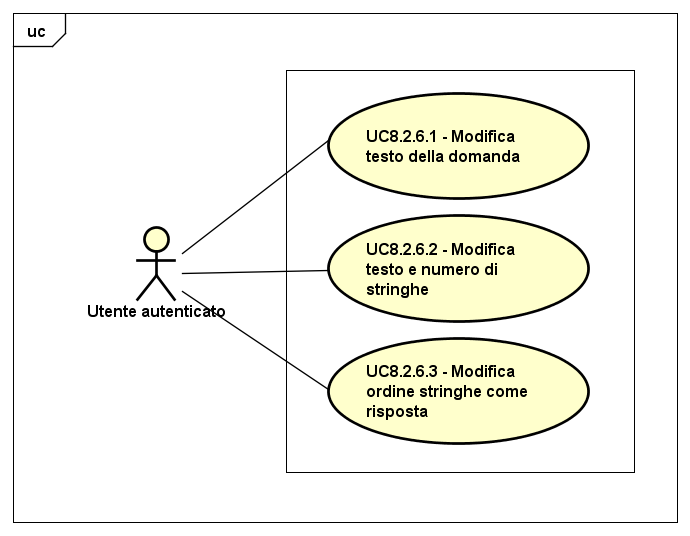
\includegraphics[scale=0.45,keepaspectratio]{UML/UC8_2_6.png}
		\caption{UC8.2.6: Modifica esercizio a riempimento di spazi vuoti}
	\end{figure}
	\FloatBarrier
	\begin{itemize}
		\item
			\textbf{Attori}: utente autenticato, utente autenticato pro;
		\item		
			\textbf{Descrizione}: l'attore può utilizzare la procedura guidata per la modifica di un esercizio a riempimento di spazi vuoti;
		\item
			\textbf{Precondizione}: il sistema ha ricevuto dall'attore la domanda da modificare;
		\item
			\textbf{Postcondizione}: l'attore ha modificato un esercizio a riempimento di spazi vuoti;
		\item
			\textbf{Scenario principale}:
	       		\begin{enumerate}
	       			\item
	       			L'attore può modificare il testo dell'esercizio (UC8.2.6.1);
	       			\item
	       			L'attore può modificare le parole che saranno sostituite con degli spazi vuoti dal sistema (UC8.2.6.2).
	 			\end{enumerate}
	\end{itemize}
	
\subsubsection{Caso d'uso UC8.2.6.1: Modifica testo dell'esercizio}
	\begin{itemize}
		\item
			\textbf{Attori}: utente autenticato, utente autenticato pro;
		\item		
			\textbf{Descrizione}: l'attore può modificare il testo dell'esercizio;
		\item
			\textbf{Precondizione}: il sistema mostra la funzionalità di modifica di un esercizio a riempimento di spazi;
		\item
			\textbf{Postcondizione}: l'attore ha modificato il testo dell'esercizio;
		\item
			\textbf{Scenario principale}: l'attore modifica il testo dell'esercizio.
	\end{itemize}


\subsubsection{Caso d'uso UC8.2.6.2: Modifica parole da oscurare}
	\begin{itemize}
		\item
			\textbf{Attori}: utente autenticato, utente autenticato pro;
		\item		
			\textbf{Descrizione}: l'attore può modificare le parole che saranno sostituite con degli spazi vuoti;
		\item
			\textbf{Precondizione}: il sistema mostra la funzionalità di modifica di un esercizio a riempimento di spazi;
		\item
			\textbf{Postcondizione}: l'attore ha modificato le parole che saranno sostituite con degli spazi vuoti;
		\item
			\textbf{Scenario principale}: l'attore modifica le parole che verranno oscurate dal sistema.
	\end{itemize}
